\chapter[Background theory and concepts]{Background theory and concepts}
In sections \ref{pedestrians} and \ref{walking} some concepts used in this research will be clarified to have unambiguous use of terms. Section \ref{puccini} will tell more about the Puccini method which is used for the design of the public space in Amsterdam. 
This chapter will be finished with summaries of related literature (section \ref{literature}) which helped forming this research and provide reference and support for the data and methods used.

\section[Pedestrians]{Pedestrians}\label{pedestrians}
\begin{description}\item[A pedestrian] is a person, by foot, with or without helping aids, that moves in the public space. The person is not a driver but a road user. Also persons with a wheelchair, rollator, roller-blades, skateboard or children's bicycle, as well as persons walking with a bike, scooter or motorbike in the hand are pedestrian according to the Wegenverkeerswet voetganger.~\cite{Crow2014}
\item[Mobility] is the freedom to choose to travel and sojourn in the public space, being able to make the trip, regardless its distance. Pedestrian mobility differs from other modes of transport, for it almost part of all other trips.~\cite{Sauter2010}
\item[Sojourning] is an important indicator for quality of public space, it includes activities as; recreational walking, waiting and hanging out in the public space.~\cite{Sauter2010} \end{description}

The Netherlands is climatic and geomorphological very favourable for walking.~\cite{Sauter2010} In cities almost all streets have two sided side-walks.~\cite{Sauter2010} Though, cycling is perceived much more important in the Netherlands as seen in the pecking order in traffic: public transport, car traffic, scooter, bicycle, pedestrian. In some regions of the Netherlands the soil is rather soft and peaty, in these circumstances the pavement has to be renewed every few years, to prevent sinking.

\subsection{Walking behaviour}\label{walking}
The rate of walking for a person is determined by many factors, environmental influences, personal influences or behaviour and biological influences. Here we focus on the environmental influences, in specific, walkability of the environment. Walkability is one of the many important determinants that influence the walking behaviour of elderly~\cite{Vine2012}. Here we try to sketch an overall overview of these determinants, according to the behaviour scheme of Bartolomew, ~\cite{Bartholmew2011} to show where walkability is positioned, next to terms like accessibility and mobility. 

The scheme in figure~\ref{behaviour} represents a small part of the personal and environmental determinants that influence the criteria for walking behaviour of elderly. It is incomplete as this is not a behaviour study, but gives a good insight in what is and is not included into the term walkability. 
First of all, the personal determinants like personal health, previous experiences and perceived self/efficiency are not part of this study. Though, what not to forget is, that these can be greatly influenced by the environmental characteristics. 

Walkability is part of the environmental determinants, terms used in dedicated studies are accessibility, walkability, safety and activity space.~\cite{Vine2012} Accessibility is the ability to access needed facilities and enable persons with disabilities to gain access through for example elevators, audio signals, walkway contours etc.
As stated in the previous section, mobility is the freedom to travel in the public space. Here we assume that all elderly have the freedom to go outside, make use of the public space and access the facilities they need.

The quality of these routes, the friendliness and the safety are gathered in the walkability determinant. So while a person in walking and accessing the public space, how user friendly and how much effort does it cost to cover these routes?

\begin{figure}[h]
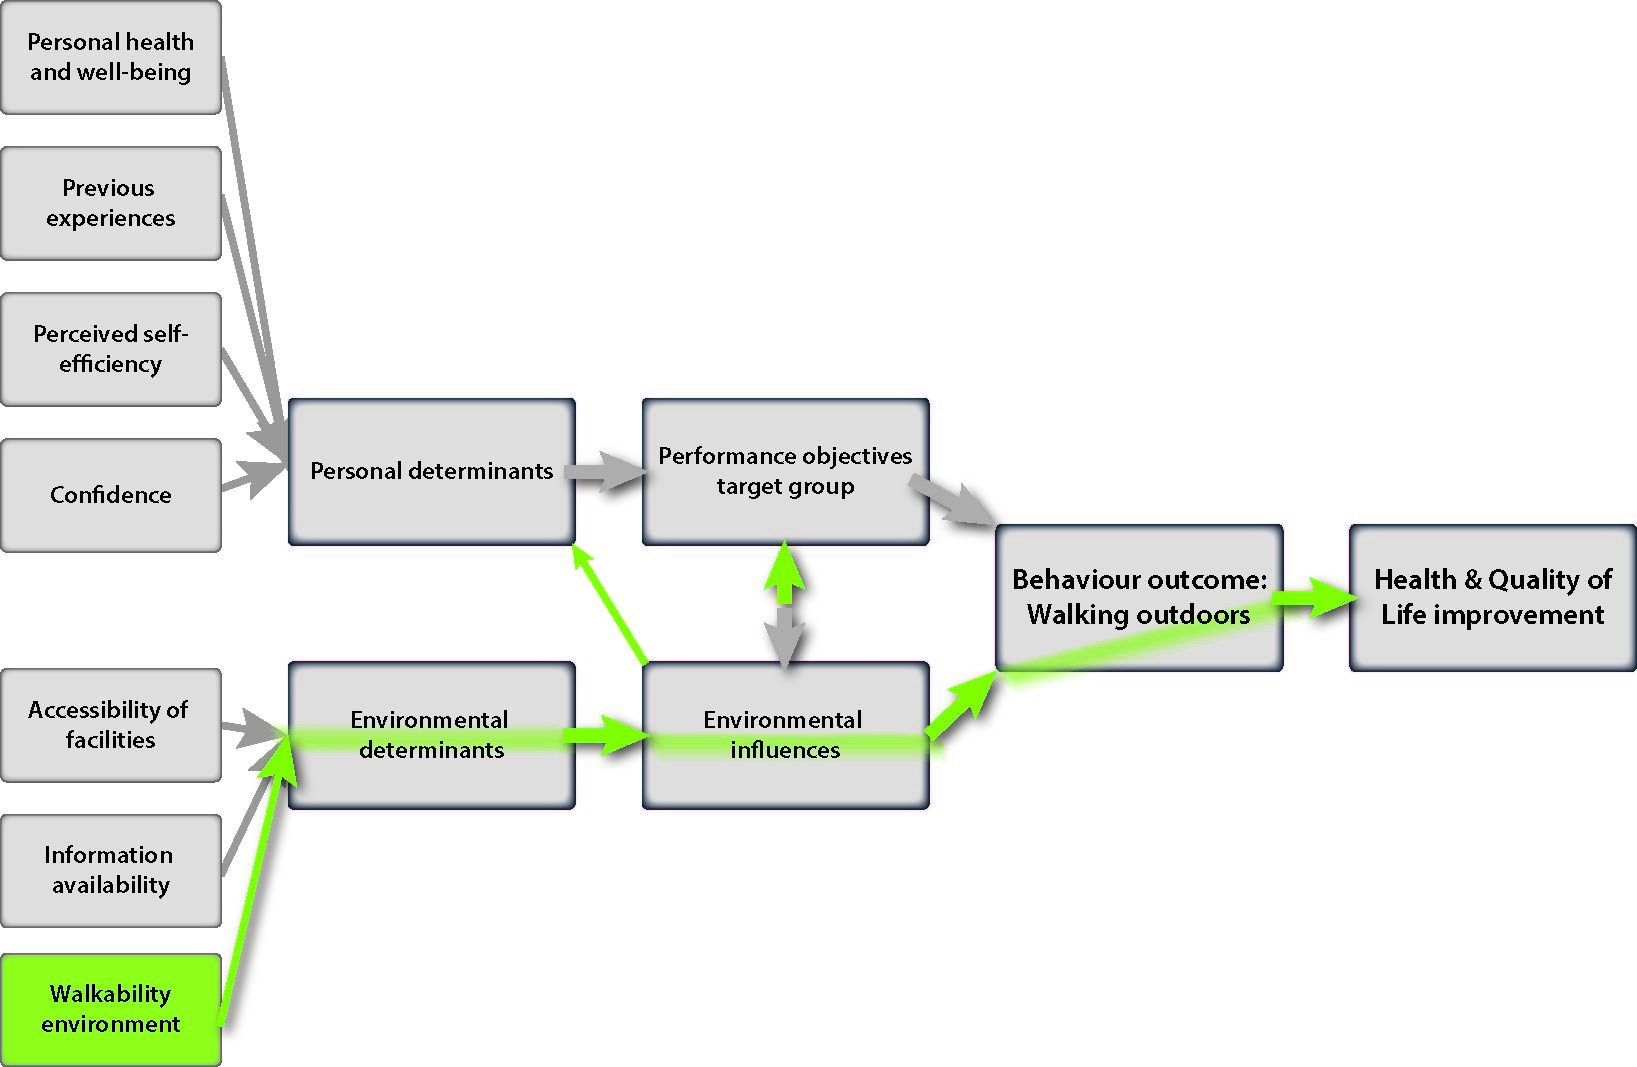
\includegraphics[width=\textwidth]{img/B_Behaviour_Scheme.jpg}
\centering
\caption[Walking Behaviour Scheme]{Walking Behaviour Scheme (Source: Boeijen, based on Bartholomew 2011)
\label{behaviour}}
\end{figure}

The individual path selection criteria of Golledge can be placed next to  this scheme to show how they influence the actual choice for walking. All the personal and environmental determinants together, make an individual decide to go by foot or not to a certain destination. Then when choosing the route and having experiences on these routes influence the choice for the next time the user wants to walk that route and which path will be followed.~\cite{Golledge2002} The individual path selection criteria by Golledge knows 3 phases: 

\begin{enumerate}
\item Choosing destinations 
\item Making a route 
\item Implementing and feedback. Confirmation or change?
\end{enumerate}  ~\cite{Golledge2002}

The first two phases are influenced by the many determinants, while the last phase provides new knowledge and experience again influencing the next time a user wants to walk outside. Increasing or decreasing the influence of the previous determinants. 


\section{Walkability factors}
From several literature studies dedicated to pedestrian-ism, elderly pedestrians, mobile impaired pedestrians, rollator users, walkability studies and walking behaviour, a list of possible walkability criteria for elderly with a rollator is created. The criteria are influenced by a wide variety of factors of the urban environment. They can be tangible and physical or intangible and more related to personal perception and feelings. ~\cite{Verschuur2014} Some criteria focused more on the broad environment of living, while others more on personal detail in the direct environment. 
Already, several other studies made an overview of walkability criteria for elderly or the mobile impaired. For example ~\cite{Verschuur2014} provides a list of parameters affecting route attractiveness and the studies in which its found. Also ~\cite{Duncan2011} provides a whole list of walkability indicators they use for calculating a walk score. Rosenberg ~\cite{Rosenberg2013} provides a summary of barriers and facilitators in the built environment. Wennberg studies a whole list of usability factors and their statistical significance, divided into categories, physical barriers, orientation and warnings, bus stops and shops, orderliness and benches and stairs. ~\cite{Wennberg2009} All these lists and other studies are used to create an own overview in order to filter out the most important walkability criteria for elderly with a rollator. This list can be found in Annex \ref{Acriteria}

For making all the criteria more orderly, they are first subdivided into tree levels of where they could occur. 

\begin{enumerate}
\item Pavement level
\item Street level
\item Environmental level
\end{enumerate}
Though, this didn't seem sufficient, some weather related and temporal issues that occur, could not be placed in this subdivision as they can occur over all these tree levels. Also crossings form a own special nice in the levels for it is not part of the pavement or the street. Therefore these are added to the tree levels mentioned above.
\begin{enumerate}
\item Weather or temporal level
\item Crossings
\end{enumerate}

Also the factors could be assigned to different categories, some had to do with accessibility and other with the quality of the environment. Five categories can be distinguished. These are inspired by ~\cite{Ballester} and ~\cite{Rosenberg2013}.

\begin{enumerate}

\item Accessibility
\item Quality 
\item Obstructions or barriers
\item Route attractiveness 
\item The feeling of safety
\end{enumerate}

Accessibility is about the access and presence of the pavements, if there is a pavement available and destinations can be reached. Some examples of factors are: the availability of public transport nodes,  availability of bridges, availability of ramps to the pavement a.o. 
The quality is about when a pavement or stair is present, what the quality is. This could include things as a non slippery pavements, the slope of bridges and the slope of the pavement. 
Obstruction contains tangible objects that are in the way, temporary or stationary.  Like protruding portals and facades, blocking commercial signs or green maintenances so branches are not hanging over the pavement.
Route attractiveness is more about the feeling one has towards the routes, the attractiveness can go down with the presence of dog droppings on the pavement, litter and garbage on the streets. While it can go up with the availability of resting benches, public toilets, green and trees along the route. 
The feeling of safety includes factors as enough time to cross the street, good overview while crossing a street, vehicle-pedestrian interaction, speed limits, presence of street lights, the amount of criminality and many others. 


\section{Puccini Method}\label{puccini}
The Puccini Method is the Amsterdam tradition for the design of the public space and formulates design principles. Public space includes all non-build-up space, open and accessible to people. The Puccini Method contains all points of policy, to the detailed design, technical details and material lists. It contains four modules, red for streets, green for vegetation, blue for water and water banks, and last, purple for street furniture, street lights and public transport stops. 
The Puccini method is the handbook for the municipality to maintain and design the public space. It is not a policy design book.~\cite{puccini2014}

The Puccini method contains 6 convictions:~\cite{puccini2014}
\begin{enumerate}
\item 	\begin{description}
		\item[Choose, not share] 
		The streets are used more intensive and pressure increases. Often the usage pressure is higher then the available physical area. Therefore the available space has to be assigned to one use, not shared. 
		\end{description}
\item \begin{description}
		\item[Simplicity and obviousness] 
		The pbulic space should be user-friendly, sustainable, strong in simplicity, timeless and obvious. With simple material and simple design, reaching for good quality.
		\end{description}
\item \begin{description}
		\item[Craft and skill as a basis] Craft expertise is the basis. Not only designing inside, but going out on the streets with work experience is the key. 
		\end{description}
\item \begin{description}
		\item[Crucial eye for detail] Detail for material use, time, financial resources and facing problems that have to be solved. 
		\end{description}
\item \begin{description}
		\item[A good plan is maintainable] After the realization of a street or square it still has to be maintained. The plan has to take the maintenance into account for the future. 
		\end{description}
\item \begin{description}
		\item[Cooperation] A lot of specialised disciplines are concerned. Throughout the whole process it is important to communicate until the end product is realized. 
		\end{description}
\end{enumerate}

Amsterdam is a cultural historic city, with many urban designs from different time periods. The historical city centre, the 19th century canal-belt, the 20-40ties en the postwar city.  The urban design has to suit the cultural historic character of the city. For every urban style zones there are material lists and standard design details.~\cite{puccini2014} A map of Amsterdam indicating where each urban time zone is located can be found in annex \ref{pucciniMap}.
	
\section{Related literature}\label{literature}
Form the few studies that do focus on elderly pedestrians some perceived as helpful for this study will be discussed in this section.
The most important researcher aiming at the elderly as a pedestrian outdoors is Agnete St\"al. The rollator is a Swedish invention, and St\"al is a Swedish researcher focussing a lot on elderly pedestrians with rollators, about their accessibility and safety in the public space and how interventions in the public space impact the elderly pedestrian.   

Literature that discusses the possible methodologies to make walkability quantifiable are often found under the term Smart Walker. The studies from Wang and Weiss  et al. focus more on the technical aspect of measuring rollator movements. 

The only study combining the pedestrians perception with measuring the helping aid is a study by Matthews at al. Though, here it is more focussed on wheelchair users, it can easily be translated to rollator users. 

\subsection{Critical walking factors for elderly with a Rollator}
Stahl is one of the few that looks at the elders perception of the built environment and how specific interventions can help rollator walks be perceived more attractive.~\cite{Stahl2008, Stahl2013}

The measurements most mentioned are:
\begin{enumerate}
\item Separation of pedestrians/cyclists
\item Lower speed limits
\item Better maintenance
\item Wider side walks
\item Decrease curb levels
\item More even surfaces on pavements
\end{enumerate}~\cite{Stahl2008}


\subsection{The Smart Walker}

There are a few researches on making a rollator more smart by using sensors; the Smart Walker. Most of these studies focus on fall protection, early warning systems or indoor navigation. There are functions such as sensor assistance, health monitoring, navigation help or cognitive assistance, obstacle avoidance and fall detection.~\cite{Wang2015} 

Most studies using an accelerometer as a sensor, calculate gait parameters such as; step length, gait cycle, step width and gait variability.~\cite{Wang2015} 

Often these studies are done in laboratory settings, using high quality sensors and sensors attached to the body.
This research aims at obstacle detection, with the help from detecting the movement of the rollator. On this, no specific literature could be found.

\subsection{Using an accelerometer for rollator monitoring}

Weiss et al. (2014) uses a smart walker to detect walking behaviour change in real time with an accelerometer mounted on the rollator.~\cite{Weiss2014} No sensor on the user is needed, but the walking behaviour is detected based on the motion transfer by the user on the walker. The goal is to identify five different classes: no movement, movement, slow, normal and fast. They confirm that walking behaviour changes can be detected by using a 3-axis accelerometer sensor on the walker.


\begin{figure}[h]
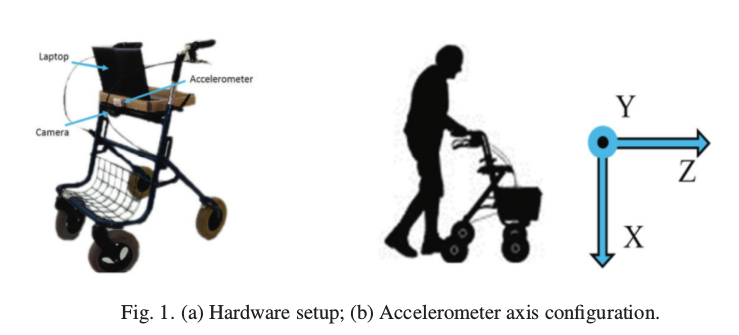
\includegraphics[width=0.75\textwidth]{img/B_Weiss.png}
\centering
\caption[Rollator with accelerometer axis configuration]{Rollator with accelerometer axis configuration. From Weiss et al.~\cite{Weiss2014} \label{rolaxis}}
\end{figure}

Wang et al. (2015) uses a standard 4-wheel rollator with a defined walking frame, where the accelerometer is positioned in the middle point between the two rear wheels. By doing this the exact distances to the wheels are know and from this the position change of the walker can be determined. By using a high cost motion capture system, the calculated trajectory's and the gait or step detection, are validated. Wang was able to calculate the displacement of the walker during every step with an accuracy of approx 1 cm.~\cite{Wang2015} By comparing a group of young adults with group of elderly people, Wang found the the walking accuracy of the elderly is lower but that step length, step period and walking speed between the two groups has no obvious difference. The classical gait indicators are not sufficient or sensitive enough to evaluate the fall risk of elderly.~\cite{Wang2015}
 
\begin{figure}[h]
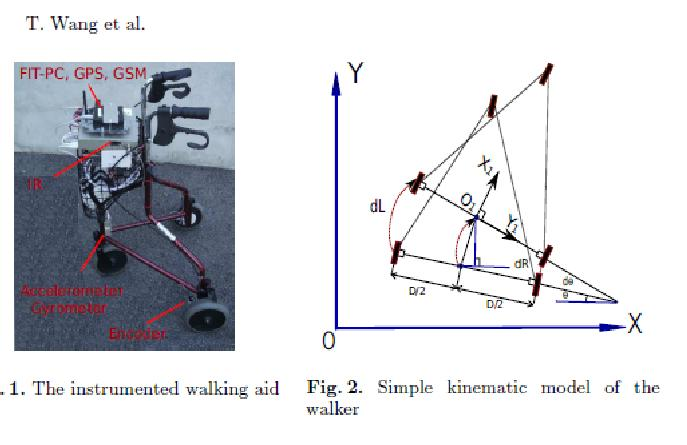
\includegraphics[width=0.5\textwidth]{img/B_Wang.jpg}
\centering
\caption[Rollator set-up]{Rollator research set-up. From Wang et al.~\cite{Wang2015} \label{rolsetup}}
\end{figure}


Both Wang and Weiss made use of a non-intrusive measurement method. Were no devices were placed on the participants but only on the rollator. 


\subsection{Outdoor quality for Wheelchair users}
Obviously, a wheeled walker and wheelchairs have a lot in common. Therefore, also literature studies aimed specific at wheelchairs can provide useful insights for rollator research. 

Matthews et al. 2003 uses a GIS based system to show that the built environment is often distorted and forms a hostile space for wheelchair users.~\cite{Matthews2003}

Small test were conducted measuring surface hindrance for wheelchair users, aiming at surface type and quality for mobility. Six common urban surfaces were tested: concrete, paving, tarmac, brick, grass and gravel. A wheelchair with occupant was pushed down a small ramp the distance rolled provides an measure for rolling resistance. 

\subsection{Elderly perception of the outdoor environment}
Ideas from Hogertz, 2010 ~\cite{hogertz2010}